\section{Data Postprocessing}

\subsection{Definition}


\begin{frame}{A typical machine learning model}
    \begin{center}
        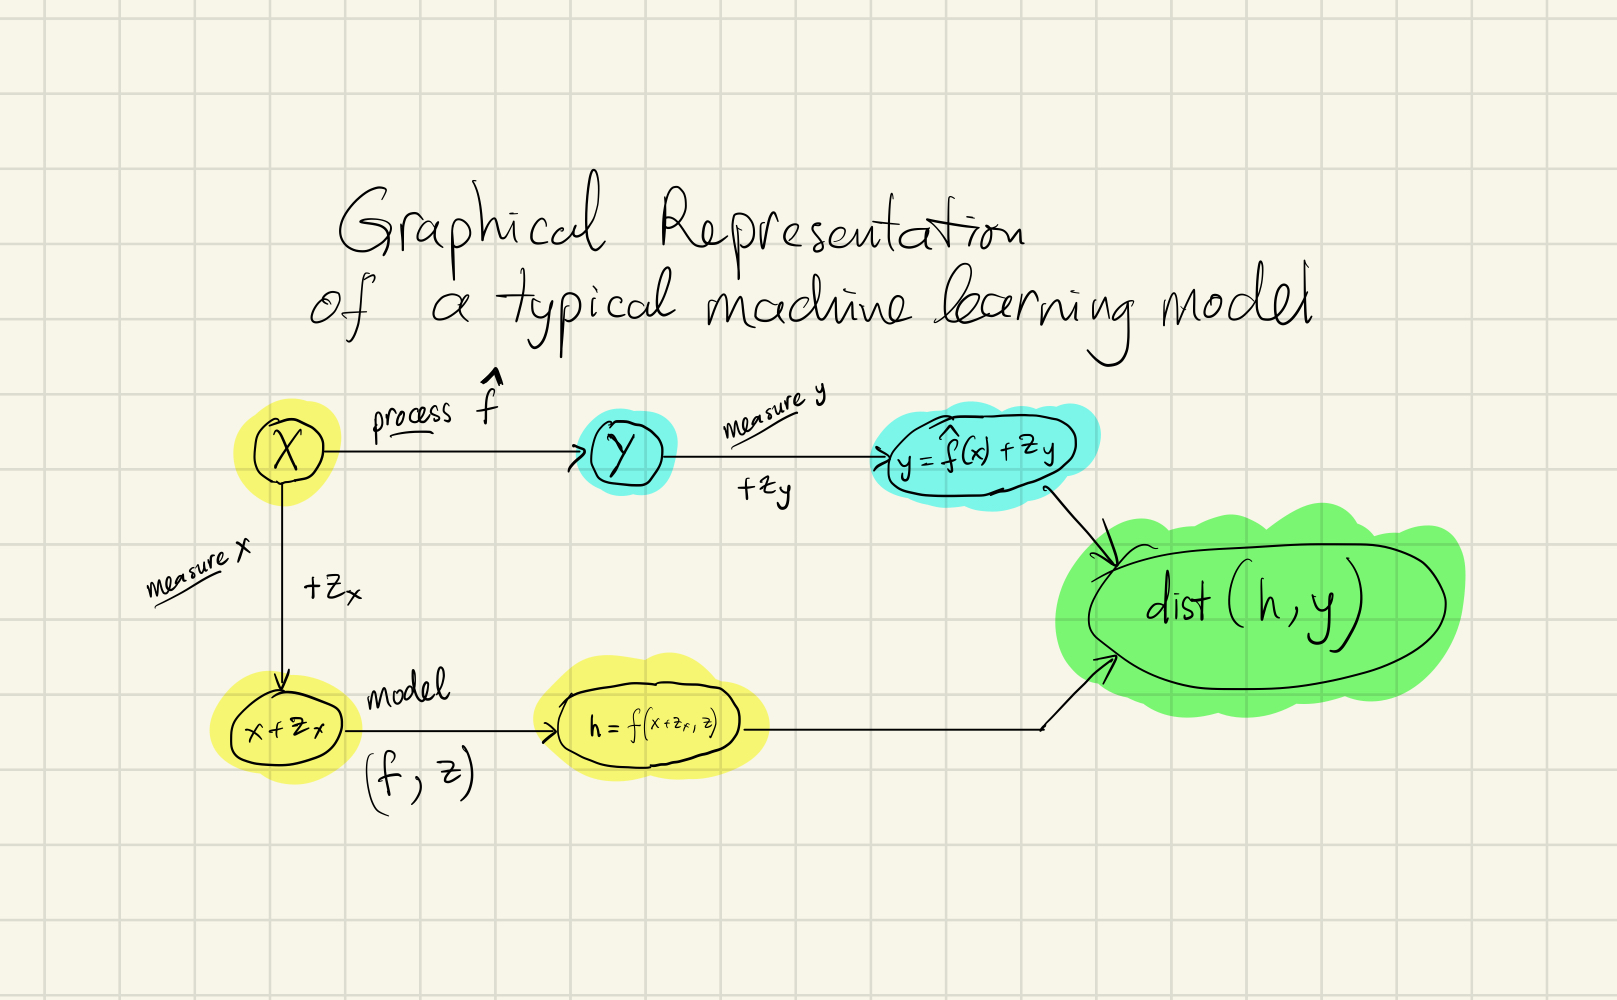
\includegraphics[width=1.0\textwidth]{assets/model.jpeg}
    \end{center}
\end{frame}

\begin{frame}{A typical machine learning model (cont)}
\begin{exampleblock}{A typical machine learning model}
Input: $x \sim X$, noise of $X$: $z_x \sim Z_x$, prediction: $h \sim H$, internal random process $z \sim Z$, model: $(f, z)$, measurement: $y = \hat{f} + z_y$, measurement noise: $z_y \sim Z_y$
\[
    h = f(x + z_x, z)
\]
\[
    y = \hat{f}(x) + z_y
\]
\[
    dist(f, \hat{f}) = \mathbb{E}_{x \sim X}[dist(h, y)]
\]

\end{exampleblock}

\begin{itemize}
    \item What is a data point? 
    \emph{A sample from $X$}
    \item What is the loss? 
    \emph{A sample from $L$}
    \item How do we know how good a model is? 
    \emph{Model Evaluation}
    \item How do we know which model is better? 
    \emph{Comparing Model}
    
\end{itemize}

\end{frame}

\subsection{Model Evaluation}

\begin{frame}{Model Evaluation}

When train a model multiple times

\begin{itemize}
    \item Losses from multiple runs are samples from distribution of loss $L$
    \item Essential to estimate the loss distribution correctly
\end{itemize}

\end{frame}

\subsection{Comparing Model}

\begin{frame}{Comparing Model}
\begin{exampleblock}{Which loss is higher?}
\begin{equation}
    u = l_{f_1} - l_{f_2}
\end{equation}
\end{exampleblock}

\begin{itemize}
    \item Evaluate a distribution? \emph{Model Evaluation}
\end{itemize}

\end{frame}